\documentclass[../stats.tex]{subfiles}
\graphicspath{{\subfix{../figures/}}}
\begin{document}
\chapter{Inference for Quantitative Data: Means}
\section{Constructing a One Sample t-Interval}
Review:
\begin{itemize}
    \item Shape 
    \begin{itemize}
        \item Normal population indicates a normal sampling distribution 
        \item $n<30$ then data needs to be stated as approximately normal.
        \item $n\geq 30$ satisfies Central Limit Theorem which guarantees approximately normal 
    \end{itemize}
    \item Center 
    \begin{itemize}
        \item As long as you are taking a random sample or using random assignment, $\mu_{\overline{x}}=\mu$
    \end{itemize}
    \item When sampling, as long as 10\% condition is met, $\sigma_{\overline{x}}=\frac{\sigma}{\sqrt{n}}$
\end{itemize}

As long as the above conditions are met, the sampling distribution of $\overline{x}: \overline{x}~N\left(\mu,\frac{\sigma}{\sqrt{n}}\right)$

When we do not know the population standard deviation (which we usually don't), we must estimate it from our sample using the sample standard deviation, $s$. However, when we do, the test 
statistic ($z$) that we previously used changes. The new test statistic is called the t-statistic and has a new distribution associated with it.

The new t-distribution is not exactly liek the standard normal curve, but it is very close:
\begin{itemize}
    \item It is still centered at 0.
    \item It is bell shaped.
    \item Its sprea dis slightly greater than the normal distribution.
    \item It has more area in the tails.
\end{itemize}
\begin{center}
    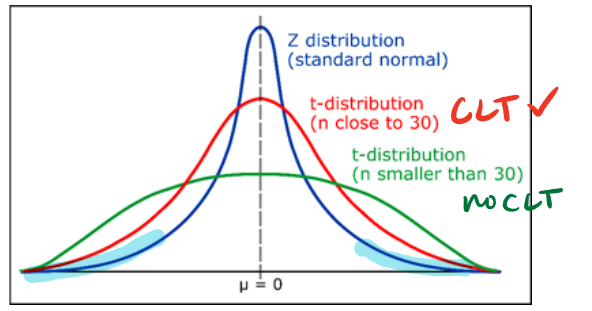
\includegraphics[width=0.8\textwidth]{7.1.1.PNG}
\end{center}
The special thing about t-distributions is the fact that it is a family of distributions. There is a unique density curve for each sample size (and the dependence on sample size is taken care of by degrees of freedom: $n-1$).

The tails on a t-distribution are ``fatter'' than a standard normal distribution. This is true because the smaller our sample size, the more variation we have, hence the fatter tails. The larger our sample size gets, the closer the t-distribution will move towards the standard normal distribution.

Constructing a Confidence Interval:
\begin{itemize}
    \item Define the Parameter
    \begin{itemize}
        \item $\mu$ = true mean of {population parameter in context}
    \end{itemize}
    \item Check the Assumptions and Conditions 
    \begin{itemize}
        \item Random: The sample should be a random sample of the population or random assignment in an experiment 
        \item Independence (10\% Condition): The sample size, $n$, must be no larger than 10\% of the population.
        \item Normality: There are multiple ways to verify this condition.
        \begin{itemize}
            \item Stated in Problem: It may be stated in the problem that the sampling distribution is approximately Normal.
            \item Central Limit Theorem: When $n$ is large, the sampling distribution of the sample means is approximately normal.
            \item Visual Representation: You are a given a graphical representation (histogram or boxplot) that depicts a shape that is approximately normal. You may also be given data that you have to graph yourself (include a sketch). You are looking for no strong skew or outliers.
        \end{itemize}
        Note: If you get a sample size less than 30, only use T-procedures if there are no outliers and no strong skew.

        \item Name the Inference Method: One Sample t-Interval 
        \item Calculate the Interval: point estimate $\pm$ margin of error 
        \[ \overline{x}\pm t^*_{n-1}\left(\frac{s}{\sqrt{n}}\right) \]
        
        To calculate $t^*_{n-1}$: 

        2nd-VARS-4:invT()
        \begin{itemize}
            \item Enter in the desired area.
            \begin{itemize}
                \item 90\% Confidence Interval: 0.95 
                \item 95\% Confidence Interval: 0.975
                \item 99\% Confidence Interval: 0.995
            \end{itemize}
            \item Enter the degrees of freedom 
            \begin{itemize}
                \item Calculation: $n-1$ where $n$ is the sample size 
            \end{itemize}
        \end{itemize}
    \end{itemize}
\end{itemize}
Write your conclusion in Context:
\begin{itemize}
    \item We are \blank\% confident that the interval from \blank to \blank captures the true mean of {population parameter in context}.
\end{itemize}
\medbreak
\begin{example}
    The Tribal Urban District Assessment (TUDA) is a government sponsored study of student achievement in large urban school districts. TUDA gives a reading test scored from 0 to 500. A score of 243 is ``basic'' reading level and a score of 281 is ``proficient.''
    Scores for a random sample of 1,470 eighth graders in a district has a mean score of 240 with a standard deviation of 42.17.

    (a) Construct and interpret a 99\% confidence interval for the mean reading test score for all of this district's eight graders.
    
    $\mu$ = true mean reading test score of all the district eight graders.

    \begin{itemize}
        \item Random: Random sample of 1470 district eighth graders.
        \item Independence: $n=1470\leq 0.10$(all of this district's eighth graders)
        \item Normal: $n=1470\geq 30$. CLT applies, so sampling dist. is approx. normal.
    \end{itemize}

    One Sample t-Interval 

    $\overline{x}\pm t^*\left(\frac{s}{\sqrt{n}}\right)$, with $t^*=2.5792$ gives interval $(237.1632,242.8368)$.

    We are 99\% confident the interval from 237.1632 to 242.8368 points captures the true mean reading test score of all the eight graders in this district.

    Using a calculator we can do the following:
    \begin{center}
        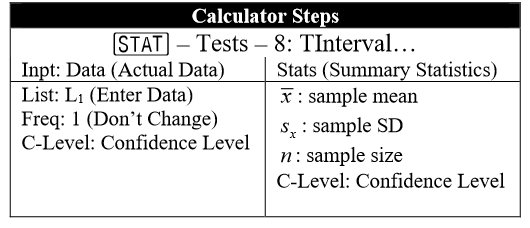
\includegraphics[width=0.8\textwidth]{7.1.2.PNG}
    \end{center}

    (b) Based on your interval, is there convincing evidence that the mean reading test score for all the eighth graders in this district is less than the basic reading level? Justify your answer using your confidence interval.

    Since our CI is entirely below 243 points there is convincing evidence that the mean reading test score is below basic reading level for all the eighth graders in this district.
\end{example}

\begin{example}
    A teacher's car records the fuel efficiency (mpg) and resets every time she fills up her gas tank. She randomly selected 20 samples of fuel efficiency from her car's computer.
    \begin{center}
        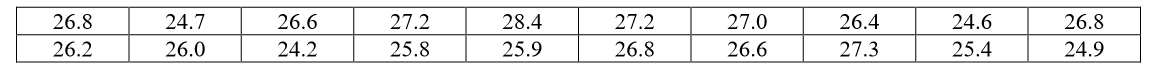
\includegraphics[width=0.8\textwidth]{7.1.3.PNG}
    \end{center}
    Given $\mu$ = true mean fuel efficiency for this teacher's car, verify the conditions for inference are met.

    \begin{itemize}
        \item Random: Randomly selected 20 fuel efficiency samples.
        \item Independence: $n=20\leq 0.10$(all car fill ups)
        \item Normal:
    \end{itemize}
    \begin{center}
        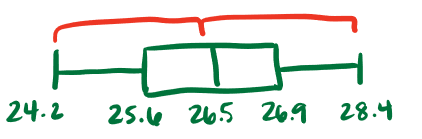
\includegraphics[width=0.8\textwidth]{7.1.4.PNG}
    \end{center}
    No strong skew or outliers so sampling distribution is approximately normal.

    To graph a boxplot with a calculator:
    \begin{itemize}
        \item STAT-Edit-1:Edit. Enter Data into L1 
        \item 2nd - Y= - Turn Plot1 On
        \item Change Type to Boxplot w/ Outliers 
        \item ZOOM-9:ZoomStat 
        \item TRACE - Identify the five number summary 
        \item Sketch on your paper - looking for no strong skew or outliers 
    \end{itemize}
\end{example}

Determing Sample Size:
\[ ME = t^{*}_{n-1}\left(\frac{s}{\sqrt{n}}\right) \]

\begin{example}
    The health teachers at a high school want to estimate the body mass index (BMI) of students at their school. The BMI of US high school students follows a normal distribution with a standard deviation of 8.1\%. How large of a sample is needed to estimate the mean BMI of this high school's students within 3\% with 98\% confidence?

    Use invT to get $t^*=2.4258$.

    Plugging this into the above formula and solving for $n$ gives $n=43$ people.
\end{example}

\section{Constructing a One Sample t-Test}
\begin{itemize}
    \item Define the parameter: $\mu$ = true mean of {population parameter in context}
    \item State the Hypotheses 
    \begin{itemize}
        \item Null Hypothesis: $H_0: \mu=\mu_0$
        \item Alternative Hypothesis: $H_A:\mu<\mu_0$, $H_A:\mu>\mu_0$, $H_A: \mu\neq \mu_0$
    \end{itemize}
    \item Check the Assumptions and Conditions 
    \begin{itemize}
        \item Randomness: The sample should be a random sample of the population or random assignment in an experiment.
        \item 10\% Condition: The sample size, $n$, must be no larger than 10\% of the population.
        \item Approx. Normal Condition: There are multiple ways to verify this condition. (These ways are the same as the one sample t-interval)
    \end{itemize}
    \item Name the Inference Method: One Sample t-Test 
    \item Calculate the Test Statistic 
\end{itemize}

The test statistic is $\text{test statistic}=\frac{\text{statistic-parameter}}{\text{standard deviation of statistic}}$

One Sample t-Test: $t=\frac{\overline{x}-\mu_0}{\left(\frac{s}{\sqrt{n}}\right)}$.

Where $\overline{x}$ is sample mean, $\mu_0$ is null mean, $s$ is sample standard deviation, and $n$ is sample size.

\begin{itemize}
    \item Obtain the p-Value 
\end{itemize}
\begin{center}
    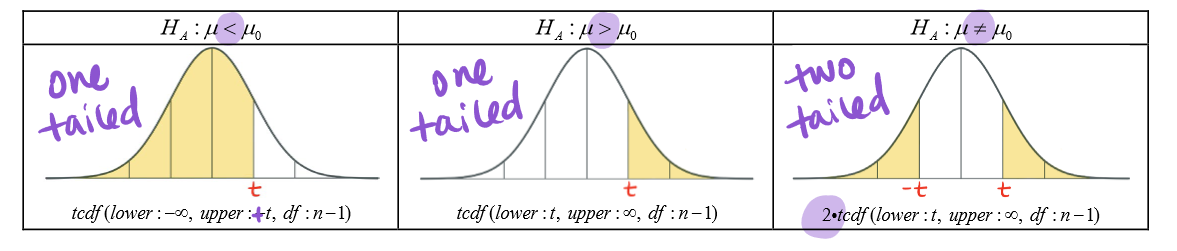
\includegraphics[width=0.8\textwidth]{7.2.1.PNG}
\end{center}

\begin{itemize}
    \item Make a Decision 
    \begin{itemize}
        \item If the p-value is less than $\alpha$, we reject the null hypothesis.
        \item If the p-value is greater than $\alpha$, we fail to reject the null hypothesis.
    \end{itemize}
\end{itemize}

State the conclusion in context: 
\begin{itemize}
    \item Since our p-value of \blank is (less/greater) than \blank, we (reject/fail to reject) the null hypothesis. There (is/is not) convincing evidence that {alternative hypothesis}.
\end{itemize}

\begin{example}
    At the Hawaii Pineapple Company, managers are interested in the sizes of the pineapples grown in the company's fields. Last year, the mean weight of the pineapples harvested from one large field was 32 ounces.
    A new irrigation system was installed in this field after the growing season. Managers wonder whether this change will affect the mean weight of future pineapples grown in the field. To find out, they select and weigh a random sample of 50 pineapples from this year's crop.
    Their sample has a mean of 31.935 ounces and a standard deviation of 2.394 ounces. Does this data give convincing evidence that the mean weight of pineapples produced in the field has changed this year?

    $\mu$ = true mean weight (ounces) of pineapples produced in this field 

    $H_0: \mu=32$, $H_A: \mu\neq 32$.

    \begin{itemize}
        \item Random: Random sample of 50 pineapples from this field 
        \item Independence: $n=50\leq 0.10$(all pineapples in this field)
        \item $n=50\geq 30$, CLT applies to sampling dist. is approx. Normal 
    \end{itemize}

    One Sample t-Test 

    $t=-0.1920$ (from the formulas above). $P(t<-1.92)=0.4243$. Since this is two tailed, $p=0.8486$.

    Since the p-value of 0.8486 is greater than $\alpha=0.05$, we fail to reject the null. There is not convincing evidence that the mean weight of pineapples produced in the field has changed this year.
\end{example}

\begin{example}
    A study was conducted on whether time perception, an indication of a person's ability to concentrate, is impaired during caffeine withdrawl. Twenty randomly selected coffee drinkers abstained from caffeine for 24 hours.
    They were asked to estimate how much time had passed during a 45-second time period. The data is displayed below.
    \begin{center}
        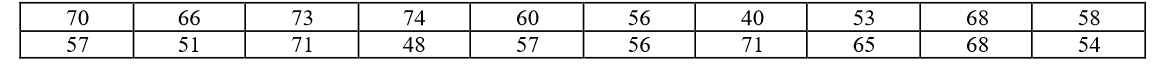
\includegraphics[width=0.8\textwidth]{7.2.2.PNG}
    \end{center}
    Is there convincing evidence at the $\alpha=0.05$ significance level that caffeine abstinence had a negative impact on time perception (causing elapsed time to be overestimated?)

    $\mu$ = true average estimation of time elapsed (seconds)

    $H_0: \mu=45$, $H_A: \mu>45$

    \begin{itemize}
        \item Random: 20 randomly selected coffee drinkers 
        \item Independence: $n=20\leq 0.10$(all coffee drinkers)
        \item Normal:
    \end{itemize}
    \begin{center}
        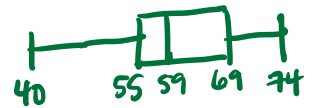
\includegraphics[width=0.8\textwidth]{7.2.3.PNG}
    \end{center}
    No strong skew or outliers, sampling dist. is approx. normal.

    One Sample t-Test 

    \begin{center}
        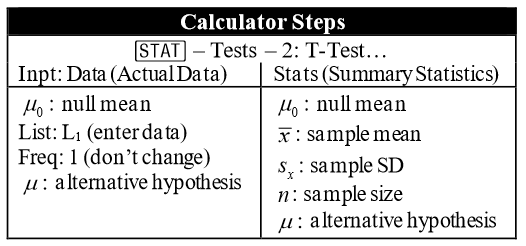
\includegraphics[width=0.8\textwidth]{7.2.4.PNG}
    \end{center}
    From this we get $t=7.5888$ and $p=0.0000002$.

    Since the p-value of 0.0000002 is less than $\alpha=0.05$, we reject the null. There is convincing evidence that caffeine abstinence had a negative impact on time perception.
\end{example}


\section{Inference for Paired Data}
Comparative studies are more convincing than single-sample investigations. For that reason, one-sample inference is less common that comparative inference. Study designs that involve making two observations 
on the same individual or one observation on each of two similar individuals, result in paired data.

When paired data result from measuring the same quantitative variable twice, we can make comparisons by analyzing the differences in each pair. If the conditions for inference are met, we can use one-sample t-procedures to perform inference about the mean difference: $\mu_D$.
These methods are called matched pairs procedures.

\begin{example}
    A researched studied a random sample of identical twins who had been separated and adopted at birth. In each case, one twin (Twin A) was adopted by a high-income family and the other (Twin B) by a low-income family. Both twins were given an IQ test as adults. Here are their scores.
    \begin{center}
        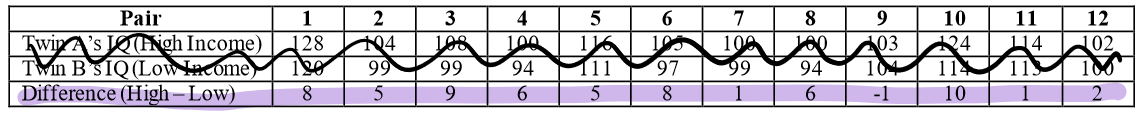
\includegraphics[width=0.8\textwidth]{7.3.1.PNG}
    \end{center}

    Construct and interpret a 95\% confidence interval for the true mean difference in IQ scores among twins raised in high-income and low-income households.

    $\mu_D$ = true mean difference in IQ scores between twins raised in high-income and low-income households.

    \begin{itemize}
        \item Random sample of 12 sets of identical twins 
        \item $n=12\leq 0.10$(all sets of identical twins)
    \end{itemize}
    Normal:
    \begin{center}
        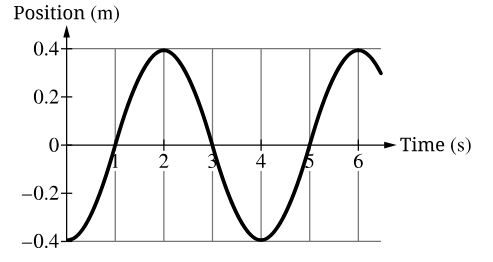
\includegraphics[width=0.8\textwidth]{7.3.2.PNG}
    \end{center}

    One Sample t-Interval for Matched Pairs.

    You can calculate using $\overline{x}_D\pm t^*_{n-1}\left(\frac{S_D}{\sqrt{n}}\right)$ or STAT-Tests-8:TInterval:

    The interval is $(2.7495, 7.2505)$.

    We are 95\% confident that the interval from 2.7495 to 7.2505 captures the true difference (High-Low) between the IQ scores of identical twins raised on high income and low income households.
\end{example}

\begin{example}
    Researchers designed an experiment to study the effects of caffeine withdrawl. They recruited 11 volunteers who were diagnosed as being caffeine dependent to serve as subjects. Each subject was barred from coffee, sodas, and other subtances 
    with caffeine during the duration of the experiment. During one two-day period, subjects took capsules containing their normal caffeine intake. During another two-days period, they took placebo capsules. The order in which the subjects took caffeine and the placebo is randomized.
    At the end of each two-day period, a test for depression was given to all 11 subjects. Researchers wanted to know whether being deprived of caffeine would lead to an increase in depression. The table displays data on the subjects' depression test scores. Higher scores show more symptoms of depression.

    \begin{center}
        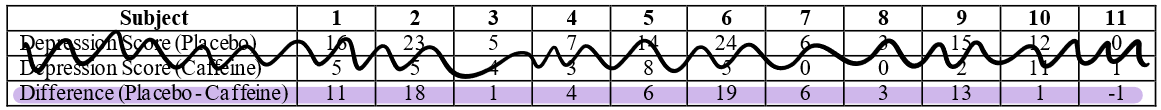
\includegraphics[width=0.8\textwidth]{7.3.3.PNG}
    \end{center}

    Does the data provide convincing evidence at the $\alpha=0.01$ significance level that caffeine withdrawl increases depression score, on average, for subjects like the ones in this experiment?

    $\mu_D$: true mean difference in depression test scores betewen normal caffeine intake and placebo capsules.

    $H_0: \mu_D = 0$, $H_A: \mu_D>0$

    \begin{itemize}
        \item Order of treatments is randomized 
        \item Assume volunteers are independent of one another 
    \end{itemize}
    \begin{center}
        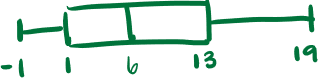
\includegraphics[width=0.8\textwidth]{7.3.4.PNG}
    \end{center}
    No strong skew or outliers so sampling dist. is approx. normal.

    One Sample t-Test for matched pairs.

    You can calculate using $t=\frac{\overline{x}_D-0}{\left(\frac{s_D}{\sqrt{n}}\right)}$ and 2nd-VARS-6:tcdf or STAT-Tests-2:T-Test 

    The $t$ value is $3.5304$ and $p=0.0027$

    Since the p-value of 0.0027 is less than $\alpha=0.01$, we reject the null. There is convincing evidence that caffeine withdrawl increases depression score, on average, for subjects like those in this experiment.
\end{example}


\section{Inference for Comparing Two Sample Means}
Constructing a Two Sample T-Interval 
\begin{itemize}
    \item Define the Parameter:
    \begin{itemize}
        \item $\mu_1$ = true mean of {population parameter in context} for {Sample 1}
        \item $\mu_2$ = true mean of {population parameter in context} for {Sample 2}
    \end{itemize}
    \item Check the Assumptions and Conditions: This is the same as for a one sample t-interval, just they have to apply for both populations.
    \item Name the Inference Method: Two Sample t-Interval for $\mu_1-\mu_2$
    \item Calculate the Interval 
    \[ (\overline{x}_1-\overline{x}_2)\pm t_{n-1}^* \left(\sqrt{\frac{(s_1)^2}{n_1}+\frac{(s_2)^2}{n_2}}  \right) \]
    Calculating the $t_{n-1}^*$ value is similar to earlier, the degrees of freedom is $n-1$ for the smaller sample size (also known as the conservative df)
\end{itemize}
\begin{itemize}
    \item Write your conclusion in context.
\end{itemize}
We are \blank \% confident the interval from \blank to \blank {units} captures the true mean difference {Pop 1-Pop 2} between {Context of Question} OR 

We are \blank\% confident that the true mean of {Pop 1 in Context} is between \blank and \blank {units} (higher/lower) than {Pop 2}
\begin{example}
    College financial aid offices expect students to use summer earnings to help pay for college. But how large are these earnings? The University of Texas studied this question by asking 
    random samples of 675 male and 621 female students with summer jobs how much they earned. Their data is summarized below.
    \begin{center}
        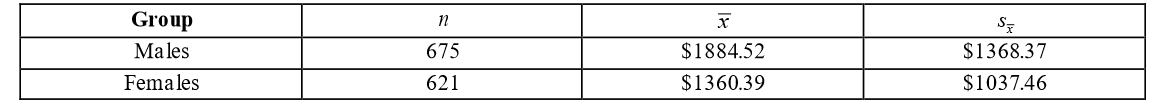
\includegraphics[width=0.8\textwidth]{7.4.1.PNG}
    \end{center}
    Construct and interpret a 90\% confidence interval for the true mean difference between summer earnings of male or female students at the University of Texas.

    $\mu_M$ = mean summer earnings of UT males, $\mu_F$ = mean summer earnings of UT females.

    \begin{itemize}
        \item Random sample of 675 male and 621 female UT students.
        \item $n_m=675\leq 0.10$(all male UT students), $n_F=621\leq 0.10$(all female UT students)
        \item $n_m=675>30$, $n_F=621\geq 30$, CLT applies, sampling dist. is approx. normal 
    \end{itemize}

    Two Sample t-Interval for $\mu_M-\mu_F$

    Using the formula above, we find that $t^* = 1.6473$, and the interval to be $(413.54,634.72)$.

    We are 90\% confident the interval from 413.62 to 634.64 dollars captures the true mean difference in summer earnings of male and female students at UT.

    To use a calculator:
    \begin{center}
        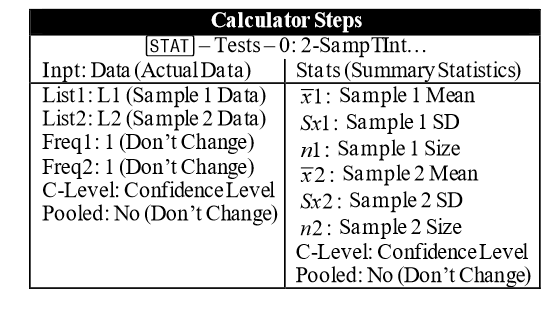
\includegraphics[width=0.8\textwidth]{7.4.2.PNG}
    \end{center}
\end{example}

Constructing a two sample t-Test 
\begin{itemize}
    \item Define the Parameter - Same as the two sample t-Interval 
    \item State the Hypotheses:
    \begin{itemize}
        \item Null Hypothesis: $H_0: \mu_1=\mu_2$
        \item Alternative Hypothesis: $H_A: \mu_1<\mu_2$, $H_A: \mu_1>\mu_2$, $H_A: \mu_1\neq \mu_2$
    \end{itemize}
    \item Check the Assumptions and Conditions: Same as two sample t-Interval 
    \item Calculate the Test Statistic
    \[ t=\frac{(\overline{x}_1-\overline{x}_2)-0}{\sqrt{\frac{(s_1)^2}{n_1}+\frac{(s_2)^2}{n_2}}} \]
    where $\overline{x}$ is sample mean, $s$ is sample standard deviation, and $n$ is sample size.

    \item Obtain the P-Value 
    \begin{center}
        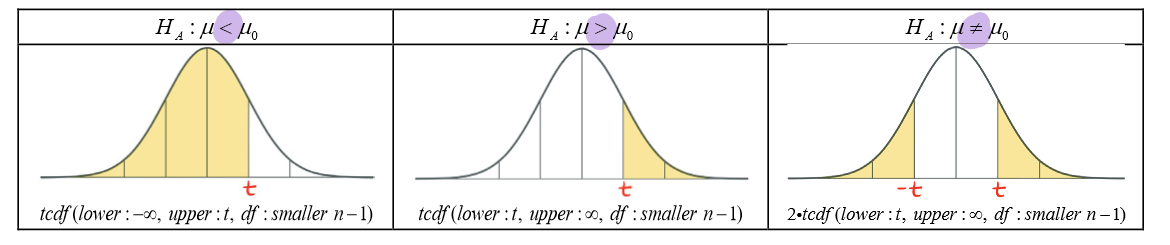
\includegraphics[width=0.8\textwidth]{7.4.3.PNG}
    \end{center}

    \item Make a Decision: You know how to do this by now 
    \item State your conclusion in Context 
    
    Since our p-value of \blank is (less/greater) than \blank, we (reject/fail to rejet) the null hypothesis. There (is/is not) convincing evidence that {alternative hypothesis}.
\end{itemize}

\begin{example}
    Many people take gingko supplements advertised to improve memory. Are these over-the-counter supplements effective? In a study, elderly adults were random assigned to the treatment group or control group. 
    The 104 participants who were assigned to the treatment group took 40 mg of gingko 3 times a day for 6 weeks. The 115 participants assigned to the control group took a placebo pill 3 times a day for 6 weeks. At 
    the end of the 6 weeks, a memory test was administered. Higher scores indicate better memory function. Summary values are given in the following table.

    \begin{center}
        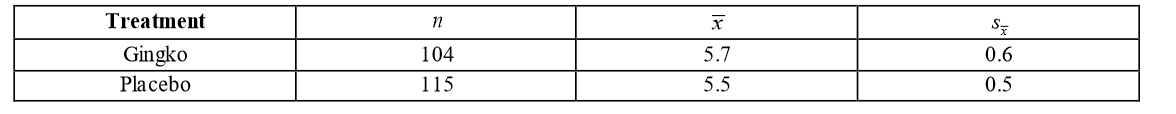
\includegraphics[width=0.8\textwidth]{7.4.4.PNG}
    \end{center}
    Based on these results, is there significant evidence that taking 40 mg of gingko 3 times a day is effective in increasing performance on a memory test?

    $\mu_G$ = mean memory score for Gingko treatment group.

    $\mu_P$ = mean memory score for placebo treatmnet group.

    $H_0: \mu_G=\mu_p$, $H_A: \mu_G>\mu_p$

    \begin{itemize}
        \item Randomly assigned elders to treatment or control group
        \item Assume independence among elderly memory test scores 
        \item $n_G=104\geq 30$, $n_p=115\geq 30$. CLT applies, sampling dist. is approx. normal.
    \end{itemize}

    Two Sample t-Test 

    Using the formula above to calculate $t$, we get $t=2.6642$, and $p=0.0045$.

    Since the p-value of 0.0045 is less than $\alpha=0.05$, we reject the null. There is convincing evidence that taking Gingko is effective in increasing memory score.

    This is how to do it in your calculator:
    \begin{center}
        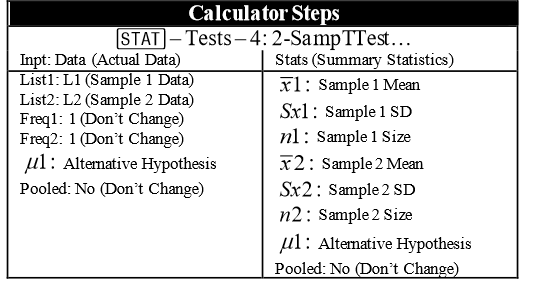
\includegraphics[width=0.8\textwidth]{7.4.5.PNG}
    \end{center}
\end{example}
\end{document}